% This is LLNCS.DEM the demonstration file of
% the LaTeX macro package from Springer-Verlag
% for Lecture Notes in Computer Science,
% version 2.4 for LaTeX2e as of 16. April 2010
%
\documentclass{llncs}
%
\usepackage{makeidx}  % allows for indexgeneration
\usepackage[pdftex]{graphicx}
\usepackage[T1]{fontenc}
\usepackage[utf8]{inputenc}
\usepackage{upquote}
%
\begin{document}
%
\mainmatter              % start of the contributions
%
\title{OCL Visualization - A Reality Check\thanks{%
      Copyright \copyright 2019 for this paper by its authors.
      Use permitted under Creative Commons License Attribution
      4.0 International (CC BY 4.0).}}
%
\titlerunning{OCL Visualization}  % abbreviated title (for running head)
%                                     also used for the TOC unless
%                                     \toctitle is used
%
\author{Edward D. Willink}
%
\authorrunning{Edward Willink} % abbreviated author list (for running head)
%
%%%% list of authors for the TOC (use if author list has to be modified)
\tocauthor{Edward Willink}
%
\institute{Willink Transformations Ltd, Reading, England,\\
\email{ed\_at\_willink.me.uk}}


\maketitle              % typeset the title of the contribution

\begin{abstract}
Visual representations, particularly in the context of a visual paradigm such as UML, have many attractions. At OCL 2018, vOCL was presented with the well intentioned goal of making hard-to-read textual OCL more accessible within diagrams. The approach as presented was unfortunately technically unsound. This paper repairs the technical problems in the vOCL approach, and contrasts it with four other approaches.

\keywords{visual programming, OCL, QVT}
\end{abstract}
%
\section{Introduction}
%
OCL~\cite{OCL-2.4} was originally part of UML, and although UML~\cite{UML-2.5} is primarily a graphical representation, OCL has remained almost steadfastly textual. %We will review a few attempts to provide a visualization of OCL.

Expression languages have been inherently textual for as long as mathematics has required expressions. FORTRAN set the standard for textual computer expression languages and apart from the introduction of objects and the "." dot operator not that much has changed since expression-wise.  Various forms of Program Flow Diagram have been attempted to provide a graphical representation. These can be quite useful in an informal context but have generally failed to contribute to a standard language; SDL~\cite{SDL} is a notable exception to this observation.

Given that graphics has generally failed for expressions, it is not surprising that graphical representations of OCL have not prospered.

The novel vOCL visualization was presented at OCL 2018 despite some concerns from the submission reviewers. More concerns were expressed during the presentation. In this paper we outline these concerns and show how they can be resolved to make vOCL a genuinely novel approach to OCL visualization.

In Section~\ref{Running Example} we present a running example and in Section~\ref{Naive AST} we present the traditional naive visualization of its OCL Abstract Syntax Tree~\cite{DragonBook}. Then in Section~\ref{vOCL} we analyse the problems in the OCL 2018 presentation of vOCL~\cite{vOCL} and solve them so that we can provide a vOCL visualization of our example. In Section~\ref{QVTs}, Section~\ref{Constraint Diagrams} and Section~\ref{Visual OCL} we present further visualizations of our running example using QVTs~\cite{QVTs}, a Constraint Diagram~\cite{Constraint-Diagrams} and Visual OCL~\cite{Visual-OCL} respectively. The characteristics of the five visualizations are contrasted in Section~\ref{Comparison}. Finally in Section~\ref{Related Work} we review the related work and conclude in Section~\ref{Conclusions}.
 
\section{Running Example}\label{Running Example}

Our running example uses the two-class example metamodel, shown in Fig~\ref{fig:ExampleMetamodel}. It is elaborated slightly, from that in vOCL~\cite{vOCL}, to add a Patient.id.

\begin{figure}
	\vspace{-10pt}
	\begin{center}
		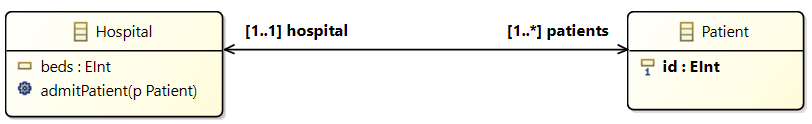
\includegraphics[width=4.5in]{Metamodel.png}
	\end{center}
	\vspace{-10pt}
	\caption{Example Metamodel}
	\label{fig:ExampleMetamodel}
	\vspace{-10pt}
\end{figure}

The metamodel shows that a \verb$Hospital$ has a number of \verb$beds$ and may serve one or more \verb$Patient$s that have an \verb$id$.

Our example OCL to be visualized comprises an invariant to check that each of the \verb$patients$ in a \verb$Hospital$ has a distinct \verb$id$.

\begin{verbatim}
context Hospital
inv uniquePatientId:
self.patients->forAll(p1, p2 | p1 <> p2 implies p1.id <> p2.id)
\end{verbatim}

(Of course, in practice, \verb|self.patients->isUnique(id)| is simpler.)

\section{Naive AST Visualization}\label{Naive AST}

The OCL specification\footnote{The OCL specification is imperfect. In this paper we use the similar classes from the Eclipse OCL Pivot model that prototypes solutions to OCL specification issues.} defines the Classes that may be used to form an Abstract Syntax Tree~\cite{DragonBook} to represent an OCL expression.

The naive AST visualization is shown in Fig~\ref{fig:NaiveUniqueIDAST}. It is auto-generated from the XMI serialization of the AST as a UML-like\footnote{Edge styling distinguishes compositions by the use bold lines with diamonds, and reference edges as dashed lines.} Object Diagram.

The diagram has been simplified to eliminate all the reference edges to, and referenced nodes for, the type/operator/property objects. It will be sufficient to study just the definition nodes. However, the diagram remains far from simple. 

It is instructive to study the diagram and to reflect upon how a reader may acquire an understanding of it.

Starting at the top of the diagram, a \verb$Class$ named \verb$Hospital$ (the context) contains a \verb$Constraint$ named \verb$uniquePatientId$ as one of its \verb$ownedInvariants$. This in turn contains an \verb$ExpressionInOCL$ as its \verb$ownedSpecification$.

The \verb$ExpressionInOCL$ contains a \verb$ParameterVariable$ named \verb$self$ as its \verb$ownedContext$. It also contains an \verb$IteratorExp$, as its \verb$ownedBody$, the root of the actual OCL expression tree.

The \verb$IteratorExp$ has further \verb$PropertyCallExp$ and \verb$OperatorCallExp$ expressions as its \verb$ownedSource$ and \verb$ownedBody$, and also two \verb$IteratorVariable$s named \verb$p1$ and \verb$p2$ as its \verb$ownedIterators$.

So far, the structure is sensibly read from top down.

\begin{figure}
	\vspace{-10pt}
	\begin{center}
		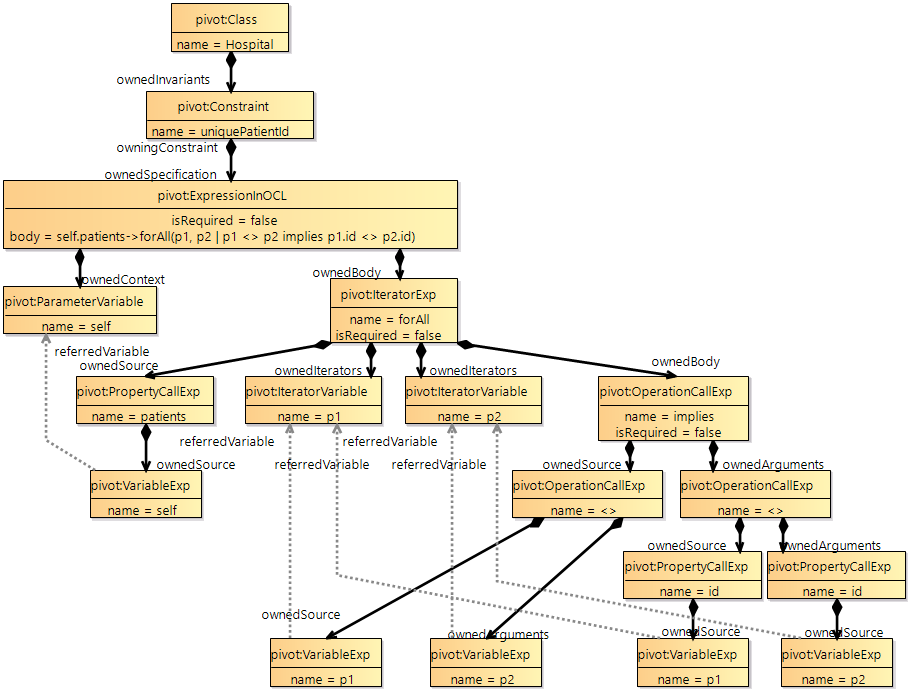
\includegraphics[width=4.8in]{UniqueIDAST.png}
	\end{center}
	\vspace{-10pt}
	\caption{Naive Visualization of Example AST}
	\label{fig:NaiveUniqueIDAST}
	\vspace{-10pt}
\end{figure}

Simple expressions such as the \verb$IteratorExp$'s \verb$ownedSource$ navigation on \verb$PropertyCallExp$ can also be read top down since we find that the navigation evaluates a \verb$patients$ property on the \verb$ownedSource$ which is a \verb$VariableExp$ named \verb$self$ referring to the overall \verb$self$ \verb$ParameterVariable$. The reader can mentally push the \verb$patients$ access on to a mental stack while discovering that \verb$self$ is the source for the \verb$patients$ navigation.

More complicated expressions cannot sensibly be read top down. If we attempt to read the \verb$IteratorExp$'s \verb$ownedBody$ top down, we encounter an \verb$implies$ \verb$OperationCallExp$ with a pair of \verb$<>$ \verb$OperatorCallExp$ expressions providing the \verb$implies$ \verb$ownedSource$ and \verb$ownedArguments$. Our mental stack needs to push three of the four top down tree paths while continuing to understand one.

If instead we attempt to understand the expression part of the tree by reading bottom up, we can start at the bottom left with a \verb$VariableExp$ named \verb$p1$ that refers to the value of the \verb$p1$ \verb$IteratorVariable$ and passes it as the \verb$ownedSource$ of the left hand \verb$<>$ \verb$OperationCallExp$. We cannot continue up since the \verb$OperationCallExp$ \verb$ownedArguments$ is not yet understood. This is resolved by yet again starting at the bottom to understand the \verb$VariableExp$ named \verb$p2$. We now have both inputs of the left-hand \verb$<>$ and may understand that the \verb$<>$ is checking that \verb$p1$ and \verb$p2$ are different and passing this up as the \verb$ownedSource$ of the \verb$implies$ \verb$OperationCallExp$. In order to fully understand the \verb$implies$ we have to go back to the bottom to understand the \verb$p1.id$ and \verb$p2.id$ navigations and \verb$p1.id <> p2.id$ comparison.

The observation that non-trivial expression trees are more easily understood by reading them bottom up is hardly surprising. An OCL evaluator can only evaluate by working bottom up, and the reader, in gaining an understanding of the OCL expression, needs to emulate that execution.

The simplified naive AST visualization requires 18 nodes and 22 edges.

\section{vOCL}\label{vOCL}

The vOCL~\cite{vOCL} visualization presented at the OCL 2018 workshop introduces some interesting novelties. By re-using the Class Diagram, vOCL avoids the need for a new programming artefact, such as an OCL document or a novel UML diagram. Each OCL constraint, pre-condition or post-condition is visualized as a `mark-up' overlay upon the pre-existing Class Diagram.

The `mark-up' comprises a sequence of directed edges from the start point (\verb$self$) to a sequence of nodes. A node for a \verb$PropertyCallExp$ may be created by drawing an ellipse or rounded rectangle around the role name text of the required property. A node for an \verb$OperationCallExp$ or \verb$IteratorExp$ may be created by drawing a new rectangle. The visualization is made more pleasing by the provision of a number of mnemonic icons for many common OCL operations.

Figure 2 of \cite{vOCL} is reproduced as Fig~\ref{fig:vOCLFig2} to demonstrate this.

\begin{figure}
	\vspace{-10pt}
	\begin{center}
		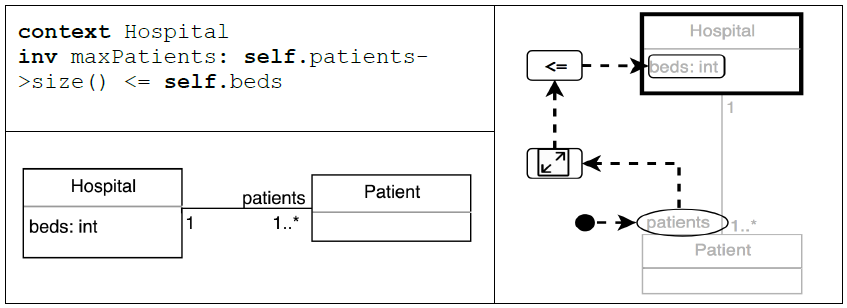
\includegraphics[width=4.5in]{vOCLFig2.png}
	\end{center}
	\vspace{-10pt}
	\caption{vOCL's Figure 2.}
	\label{fig:vOCLFig2}
	\vspace{-10pt}
\end{figure}

At top left, we see the OCL constraint to be visualized. At bottom left, we see the Class Diagram for the metamodel. At the right we see the `mark-up' in black upon the metamodel in grey.

The black box for \verb$Hospital$ identifies it as the context and consequently the \verb$self$ object when we start to read at the black filled circle.

The first arrow takes us from \verb$self$ to \verb$patients$ giving us \verb$self.patients$.

The next arrow takes us to the icon for the \verb$size()$ operator giving us \verb$self.patients.size()$.

Then on to the icon for the \verb$<=$ operator giving us \verb$self.patients.size() <=$.

Now we hit the problem. We continue on from the \verb$<=$ to the rounded rectangle around \verb$Hospital.beds$. Why does the result of a Boolean \verb$<=$ contribute to the evaluation of \verb$Hospital.beds$? Where is the missing second input to \verb$<=$? Where does the Boolean result of \verb$<=$ go to?

If we look at the naive AST visualization of this expression shown in Fig~\ref{fig:NaiveInvAST} and the equivalent mark-up for the reading order in green, the problem gets a little clearer.

\begin{figure}
	\vspace{-10pt}
	\begin{center}
		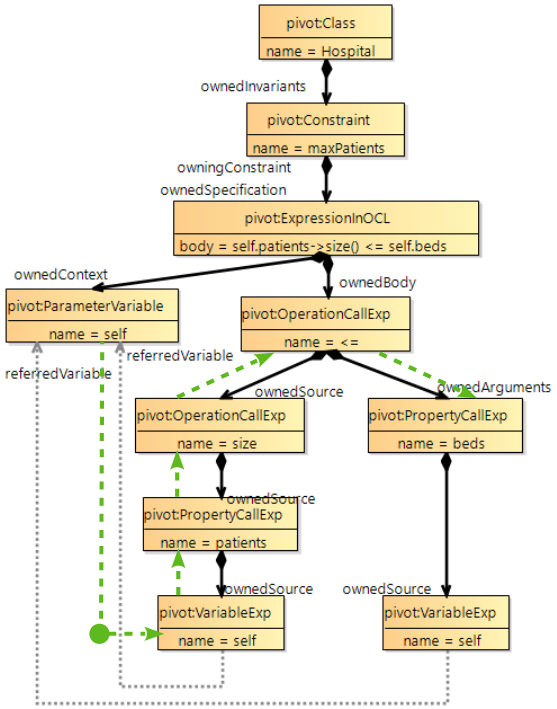
\includegraphics[width=3.5in]{vOCLInvASTOverlay.png}
	\end{center}
	\vspace{-10pt}
	\caption{Naive Visualization of vOCL invariant}
	\label{fig:NaiveInvAST}
	\vspace{-10pt}
\end{figure}

The AST comprises a \verb$<=$ \verb$OperationCallExp$, whose left-hand \verb$ownedSource$ is the chain of \verb$VariableExp$, \verb$PropertyCallExp$, \verb$OperationCallExp$ to evaluate \verb$self.patients.size()$ and the right hand side is the shorter chain for \verb$VariableExp$, \verb$PropertyCallExp$ for \verb$self.beds$.

It can be seen that the reading order defined by the arrows in Fig~\ref{fig:vOCLFig2} take us up the left hand expression in bottom up fashion to the \verb$<=$, but then top down on the right hand side without ever visiting the \verb$self$ \verb$VariableExp$. For this simple case, intuition might perhaps suggest that \verb$self$ was implicit as the self-container of the \verb$beds$ rounded rectangle. However, in more complex cases magic rather than intuition is required to explain the semantics.

Unfortunately the vOCL paper does not really define the semantics of its reading order arrow. Rather its table provides `Navigational arrow to follow the constraint'. If `navigational' is meant in the modelling sense of navigation from one class via a Property to another, at most one of the four arrows in Fig~\ref{fig:vOCLFig2} is `navigational'.

When this paper was presented at OCL 2018, the intuitive nature of reading order and the inability of this representation to handle multiple instances of the same type seemed to make this approach unsound. However if we permit multiple start points, and define the reading order arrow as the data flow in the expression AST, both these problems are solved as shown in green on Fig~\ref{fig:FixedvOCLFig2}.

\begin{figure}
	\vspace{-10pt}
	\begin{center}
		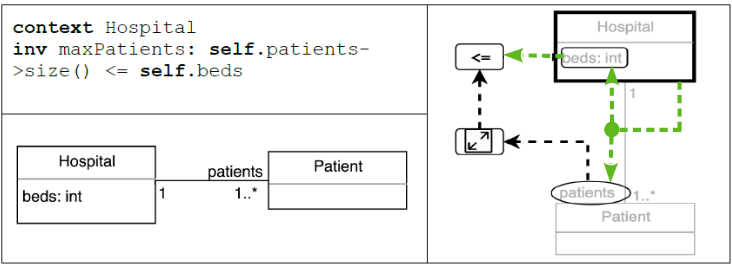
\includegraphics[width=4.5in]{FixedvOCLFig2.png}
	\end{center}
	\vspace{-10pt}
	\caption{Fixed vOCL's Fig 2.}
	\label{fig:FixedvOCLFig2}
	\vspace{-10pt}
\end{figure}

The corresponding AST of this `mark-up' is shown in Fig~\ref{fig:FixedNaiveInvAST}.

\begin{figure}
	\vspace{-10pt}
	\begin{center}
		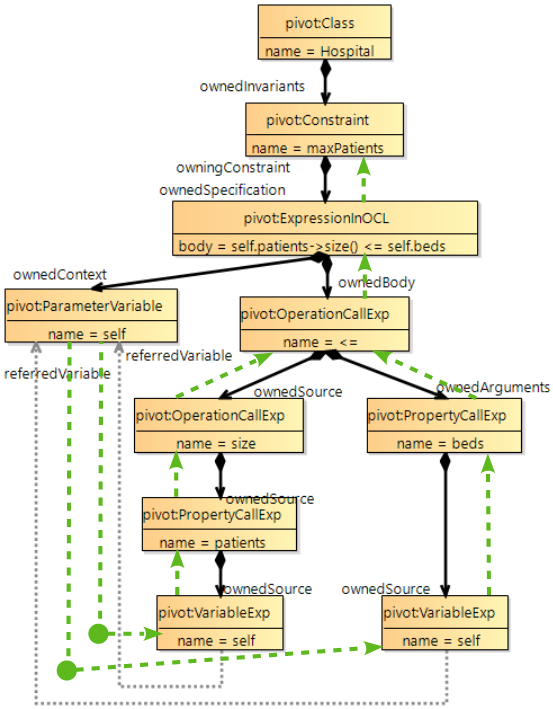
\includegraphics[width=3.0in]{FixedvOCLInvASTOverlay.png}
	\end{center}
	\vspace{-10pt}
	\caption{Fixed Naive Visualization of vOCL invariant}
	\label{fig:FixedNaiveInvAST}
	\vspace{-10pt}
\end{figure}

Once we can have multiple instances, and the reading order is clear, we can solve our example as shown in Fig~\ref{fig:vOCLinv}. The three blobs correspond to the three variables \verb$self$, \verb$p1$ and \verb$p2$, and each contributes a partial reading. Since we have multiple blobs, it is no longer sensible to use grey for the background metamodel so that the one self blob can be black.

The isolated blob for \verb$self$ is bound to \verb$Hospital$ and reads as \verb$self.patients$ to make available a \verb$Patient$ for binding to each of the other two blobs, one for \verb$p1$ and one for \verb$p2$.

One pair of readings from \verb$p1$ and \verb$p2$, passes via the \verb$<>$ operation to the \verb$self$ input of \verb$implies$. Another pair of readings passes via an \verb$id$ navigation to another \verb$<>$ operation that provides the other \verb$implies$ input. The lack of an \verb$implies$ output can be interpreted as a short form for must-be-true. Note that there are two rounded rectangles around the \verb$Patient.id$ property, one for each of \verb$p1.id$ and \verb$p2.id$.

\begin{figure}
	\vspace{-10pt}
	\begin{center}
		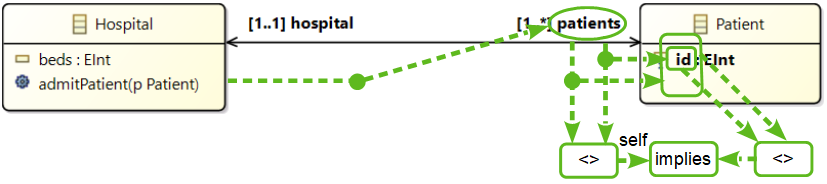
\includegraphics[width=4.0in]{vOCLinv.png}
	\end{center}
	\vspace{-10pt}
	\vspace{-10pt}
	\caption{Fixed vOCL for Running Example.}
	\label{fig:vOCLinv}
	\vspace{-10pt}
\end{figure}

The vOCL realization requires 9 nodes and 12 edges. The savings arise from re-use of the UML elements and from folding \verb$Variable$ and \verb$VariableExp$ nodes onto a starting blob.

\section{QVTs Visualization}\label{QVTs}

The Eclipse QVTd project provides an alternative form of OCL visualization. This facilitates visualization of the matching and subsequent reactions of a schedulable rule. The embedding of our example in QVTr is shown below:

\begin{verbatim}
top relation isOk {
  domain from h1 : Hospital {} {
    h1.patients->forAll(p1, p2 | p1 <> p2 implies p1.id <> p2.id)
  };
  enforce domain to h2 : Hospital {};
}
\end{verbatim}

The outer relation just transforms the \verb$h1$ instance of \verb$Hospital$ to the \verb$h2$ instance. Our example is embedded as a guard that inhibits conversion if the patient id's are not unique. The UML-like QVTs visualization is shown in Fig~\ref{fig:QVTs}.

\begin{figure}
	\vspace{-10pt}
	\begin{center}
		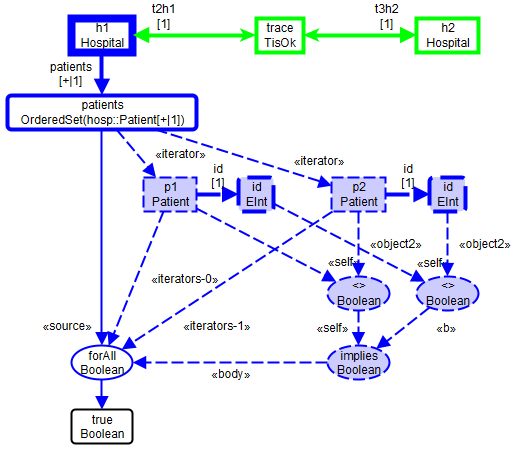
\includegraphics[width=4.0in]{QVTs.png}
	\end{center}
	\vspace{-10pt}
	\caption{QVTs Visualization of Example}
	\label{fig:QVTs}
	\vspace{-10pt}
\end{figure}

The top row shows the QVT functionality matching an \verb$h1$ \verb$Hospital$ instance for conversion to an \verb$h2$ instance via a \verb$trace$ instance. Only \verb$h1$ is relevant for discussing the OCL visualization.

The thick solid line from \verb$h1$ to \verb$patients$ shows the navigation via the \verb$patients$ property from the rectangular \verb$Hospital$ Class-instance named \verb$h1$ to the rounded-rectangular \verb$OrderedSet$ of \verb$Patient$ DataType-valued named \verb$patients$.

The thin solid line labelled \verb$«source»$ from \verb$patients$ to the \verb$forAll$ ellipse, shows the use of \verb$patients$ as the source of a \verb$forAll$ iteration. The two iterators are shown as rectangles named \verb$p1$ and \verb$p2$, linked by edges labelled \verb$«iterator»$ from the domain of the iteration and by edges labelled as \verb$«iterators-0»$ and \verb$«iterators-1»$ to the \verb$forAll$ to which they contribute. The remaining input of the \verb$forAll$ labelled \verb$«body»$ provides the result of the body expression of the iteration. Each of the \verb$p1$ and \verb$p2$ iterators are an input to an ellipse of a \verb$<>$ operation that feeds the \verb$«self»$ input of the \verb$implies$ operation that provides the iteration body. Each of the \verb$p1$ and \verb$p2$ iterators also provides the source to a corresponding navigation of the \verb$id$ property whose value is passed via the other \verb$<>$ operation to the \verb$b$ input of the \verb$implies$.

Finally the thin solid line from the \verb$forAll$ iteration to the \verb$true$ literal imposes the constraint that the result of the \verb$forAll$ must be \verb$true$ for the overall QVTs rule to be permitted to execute.

Most of the elements use thin lines indicating that they are expressions whose value is checked, rather than objects whose existence forms part of the pattern match. The lines are also dashed rather than solid indicating that there may be zero or many computations to be performed. In this example the dashed lines correspond to the iteration body that may be separately evaluated for each iterator permutation. Conversely the solid line shows that the three h1-patients-forAll-true edges are always evaluated/matched exactly once.

The QVTs is a domain-specific visualization focussed on the objects/values. All OCL constructs can  be visualized. The visualization is auto-generated and may only be edited to provide a more aesthetically pleasing layout.

Our example requires 11 nodes and 15 edges. The savings are mostly due to folding the VariableExp nodes that access a value into the Variable that provides the value.

\section{Constraint Diagrams}\label{Constraint Diagrams}

Constraint Diagrams~\cite{Constraint-Diagrams} are a Constraint rather than an OCL visualization. Fig~\ref{fig:ConstraintDiagram} shows our example.

\begin{figure}
	\vspace{-10pt}
	\begin{center}
		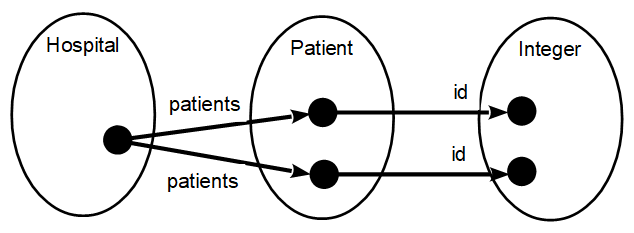
\includegraphics[width=3.5in]{ConstraintDiagram.png}
	\end{center}
	\vspace{-10pt}
	\caption{Constraint Diagram Visualization of Example}
	\label{fig:ConstraintDiagram}
	\vspace{-10pt}
\end{figure}

The ability of the notation to depict membership of domains is well suited to this example.

The left hand ellipse depicts the domain of \verb$Hospital$ instances, with a single instance shown by the blob.

The middle ellipse depicts the domain of \verb$Patient$ instances with two distinct instances shown by two distinct blobs. Each blob is related to the \verb$Hospital$ instance by the \verb$patients$ relationship.

The right hand ellipse depicts the domain of \verb$Integer$ values with two distinct values shown by two distinct blobs. Each blob is related by the \verb$id$ relationship to a correspondingly distinct \verb$Patient$ instance.

While the notation is clearly not OCL, it is visualizing the same concepts. Blobs correspond to instances, edges to property navigations. Distinctness of the blobs realises the \verb$<>$ operation almost invisibly. Multiple blobs realize the dual \verb$forAll$ very elegantly. The \verb$implies$ operation is also invisible, arguably because the Constraint Diagram implements a slightly different logic; the possibility that the iterators are the same is just not possible.

This example demonstrates how Constraint Diagrams have a `sweet spot' that can often coincide with typical usage. However when something else is required more complexity is needed. There is no support for arbitrary OCL.

The example requires 8 nodes and 4 edges. There is very little extra text.

\section{Visual OCL}\label{Visual OCL}

Visual OCL re-uses typical UML graphical idioms for its visualization, particularly the compartment nesting for hierarchical state machines. Fig~\ref{Visual OCL} shows our example. (The figure is an adaptation of Fig~2.32 of \cite{Visual-OCL}.)

\begin{figure}
	\vspace{-10pt}
	\begin{center}
		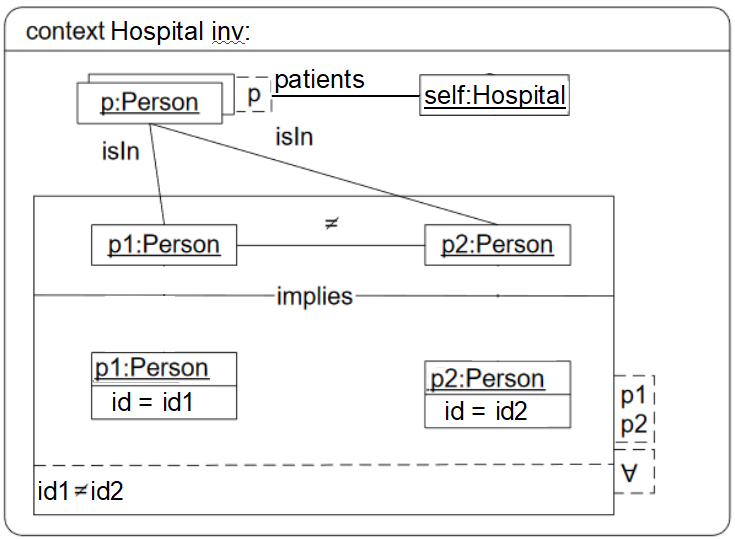
\includegraphics[width=3.5in]{VisualOCLinv.png}
	\end{center}
	\vspace{-10pt}
	\caption{Visual OCL Visualization of Example}
	\label{fig:VisualOCL}
	\vspace{-10pt}
\end{figure}

The outer compartment is top-titled to show that it is an invariant of a \verb$Hospital$. It contains a side-titled compartment for a $\forall$ with \verb$p1$ and \verb$p2$ iterators. This in turn contains a pair of compartments for left and right hand side of an \verb$implies$ operation. The lower compartment is split so that a textual expression can express what cannot be expressed graphically.

Within most of the compartments, a small UML pattern identifies a part of the expression.

In the outer compartment, a self instance of \verb$Hospital$ has a \verb$patients$ navigation to the \verb$p$ multi-instance of Patient.

The top half of the \verb$implies$ identifies two \verb$Person$ instances named \verb$p1$ and \verb$p2$ with a $\neq$ relationship between them, and the special \verb$isIn$ relationship to the outer \verb$Person$ multi-instance.

The bottom half of the \verb$implies$ again shows the two \verb$p1$ and \verb$p2$ \verb$Person$ instances but now with identification of the \verb$id$ attributes, whose value is constrained by the $\neq$ in the textual box.

Given a particularly helpful UI, it is perhaps possible to draw the diagram with 12 node/compartment creations, 3 edge creations and 10 text token selections/entries.

Contrasting Visual OCL with the naive visualization suggests that the main difference is that the compositions of the naive visualizations are replaced by compartment nesting. Since both compositions and compartments are limited to a single parent, the use of nested compartments seems sound and so the only limitation is in the diversity of helpful idioms such as the $\forall$ iteration side-titling and a guarantee that whatever lacks a special idiom can be captured by a textual compartment.

In the example, use of $\forall$ and $\neq$ rather than \verb$forAll$ and \verb$<>$ illustrates a dilemma that has been resolved  by favouring a mathematical notation rather than the OCL which is itself a compromise between compactness for mathematicians and readability for casual programmers. Not following OCL seems like a mistake since ultimately the textual compartment should be OCL rather than OCL-like.

\section{Comparison}\label{Comparison}

The characteristics of the five visualizations are summarized in the following table.

\begin{center}
	\begin{tabular}{|| c || c | c | c | c | c ||} 
		\hline
		\hline
		Visualization & Nodes & Edges & Texts & OCL Coverage & Diagram Editing \\ 
		\hline
		\hline
		Naive AST & 19 & 22 & - & Full & Auto-generated \\ 
		\hline
		vOCL & 9 & 12 & - & Full & Mark-up \\ 
		\hline
		QVTs & 11 & 15 & - & Full & Auto-generated \\ 
		\hline
		Constraint Diagram & 8 & 4 & - & Partial & Manual Edit \\ 
		\hline
		Visual OCL & 12 & 3 & 10 & Full & Manual Edit \\ 
		\hline
		\hline
	\end{tabular}
\end{center}

The nodes and edges indicate how many graphical artefacts are used by the visualization of our running example. For most of the visualizations, the text is rendered automatically from metamodel elements. Only for Visual OCL does additional text appear to need manual entry.  

The Constraint Diagram has distinctly lower artefact counts, but it has only partial coverage of OCL syntax. Our running example may be unfairly well suited to a Constraint Diagram visualization.

Two of our visualizations are secondary; they are auto-generated from the textual OCL or from QVTr. The other three are primary, requiring an appropriate graphical editor. vOCL requires an ability to mark up a standard UML Class Diagram. The remaining two require editing support for a new kind of Diagram.

The need for new editing capabilities is unattractive, but even the auto-generated visualizations need improved tooling to provide adequate layouts. The figures in this paper required considerable manual enhancement.

\section{Related Work}\label{Related Work}

This paper was motivated by a need to solve the problems in vOCL~\cite{vOCL}. The solutions and examples are presented here in Section~\ref{vOCL}.

We identify the Dragon Book~\cite{DragonBook} as a source for the traditional naive AST visualization.

Alternative visualizations have been provided as Constraint Diagrams~\cite{Constraint-Diagrams} and as Visual OCL~\cite{Visual-OCL}. We provide examples of these diagrams in Section~\ref{Constraint Diagrams} and Section~\ref{Visual OCL}.

We identify a more modern OCL visualization embedded within the QVTs visualization of the Eclipse QVTd project~\cite{Eclipse-QVTd}.

Overall our comparison of five alternative visualizations is as inconclusive as the two contrasted in ~\cite{two-OCLs}.

\section{Conclusions}\label{Conclusions}

We have remedied the deficiencies in vOCL so that its `navigation' arrows have a consistent data flow semantic, and so that multiple start points can accommodate non-trivial expressions.

We have presented five alternative visualizations of an OCL expression of moderate complexity. It is far from clear that any of the visualizations is unambiguously better than any other. Each can be good for a particular usage.

vOCL and Constraint Diagrams may be better within a UML tool, but the attempt to hide OCL completely seems unrealistic, since OCL must be used when the expression gets too complex. The new graphical idioms therefore just add to the amount to learn and require tooling to provide new diagrams. 

%
% ---- Bibliography ----
%
\begin{thebibliography}{}
%
%\bibitem{zzOCL-Determinism}
%Gogolla, M., Hilken, F.: Making OCL Collection Operations More Deterministic with Restricting Equations, 16th International Workshop in OCL and Textual Modeling, October 2, 2016, Saint-Malo, France.
%\url{http://www.db.informatik.uni-bremen.de/publications/intern/ocl2016-talk-lightning-mg-fh.pdf}

%\bibitem{zzLazy OCL}
%Tisi, M., Douence, R., Wagelaar, D.: Lazy Evaluation for OCL.
%15th International Workshop on OCL and Textual Modeling, September 8, 2015, Ottawa, Canada.
%\url{https://ocl2015.lri.fr/OCL\_2015\_paper\_1111\_1115.pdf}

%\bibitem{zzOCL-CG}
%Willink, E.: An extensible OCL Virtual Machine and Code Generator.
%2012 Workshop on OCL and Textual Modelling (OCL 2012), September 30, 2012, Innsbruck, Austria.
%\url{http://st.inf.tu-dresden.de/OCL2012/preproceedings/14.pdf}

%\bibitem{zzWillink-EXE2016}
%Willink, E: Local Optimizations in Eclipse QVTc and QVTr using the Micro-Mapping Model of Computation,
%2nd International Workshop on Executable Modeling, Exe 2016, Saint-Malo, October 2016.
%\url{http://eclipse.org/mmt/qvt/docs/EXE2016/MicroMappings.pdf}

%\bibitem{zzSafe OCL}
%Willink, E.: Safe Navigation in OCL.
%15th International Workshop on OCL and Textual Modeling, September 8, 2015, Ottawa, Canada.
%\url{https://ocl2015.lri.fr/OCL\_2015\_paper\_1111\_1400.pdf}

%\bibitem{zzDresden-OCL}
%Dresden OCL Project.\\
%\url{http://www.dresden-ocl.org/index.php/DresdenOCL}

%\bibitem{zzEclipse-OCL}
%Eclipse OCL Project.\\
%\url{https://projects.eclipse.org/projects/modeling.mdt.ocl}

%\bibitem{zzQVT-1.3}
%OMG. Meta Object Facility (MOF) 2.0 Query/View/Transformation Specification, Version 1.3.
%OMG Document Number: ptc/16-06-03, June 2016.

%\bibitem{zzUSE}
%USE, The UML-based Specification Environment. \url{http://useocl.sourceforge.net/w/index.php/Main\_Page}

\bibitem{DragonBook}
Aho, A., Sethi, R., Ullman, J.: Compilers, Principles, Techniques and Tools, Addison Wesley, 1986

\bibitem{vOCL}
Badreddin, O., Barraza, G., Hamou-Lhadj, A.: vOCL: A novel approach for UML constraints modeling, 18th International Workshop in OCL and Textual Modeling, October 14, 2018, Copenhagen, Denmark. \url{http://ceur-ws.org/Vol-2245/ocl\_paper\_7.pdf}

\bibitem{two-OCLs}
Fish, A., Howse, J., Taentzer, G., Winkelmann, J.: Two visualizations of OCL: a comparison. Brighton, UK, 2005. \url{https://research.brighton.ac.uk/files/186722/VOCLTR.pdf}

\bibitem{Constraint-Diagrams}
Kent, S.: Constraint Diagrams: Visualizing Invariants in Object-Oriented Models. OOPSLA 1997. \url{https://www.cs.kent.ac.uk/pubs/1997/794/content.pdf}

\bibitem{Visual-OCL}
Kiesner, C., Taentzer, G., Winkelmann, J.: Visual OCL: A Visualization of the Object Constraint Language, TU Berlin Technical Report 2002/23, 2002. \url{http://www.user.tu-berlin.de/o.runge/tfs/projekte/vocl/gKTW02.pdf}

\bibitem{SDL}
Rockstrom, A., Saracco, R.: SDL-CCITT Specification  and  Description  Language,IEEE Transactions on Communications 30(6):1310 - 1318, July 1982, \url{https://www.researchgate.net/publication/224733068\_SDL-CCITT\_specification\_and\_description\_language}

\bibitem{QVTs}
Willink, E.: QVTs: A TGG-like graphical representation for efficient Declarative Model to Model Transformation scheduling, March 2019, \url{https://www.eclipse.org/mmt/qvt/docs/ICGT2019/GraphicalQVT.pdf}

\bibitem{UML-2.5}
OMG Unified Modeling Language (OMG UML), Version 2.5, {OMG Document Number}: formal/15-03-01, Object Management Group (2015), \url{http://www.omg.org/spec/UML/2.5}

\bibitem{OCL-2.4}
Object Constraint Language. Version 2.4., OMG Document Number: formal/2014-02-03, Object Management Group (2009),  \url{http://www.omg.org/spec/OCL/2.4}

\bibitem{Eclipse-QVTd}
Eclipse QVT Declarative Project.\\
\url{https://projects.eclipse.org/projects/modeling.mmt.qvtd}

\end{thebibliography}
\end{document}
